%%%%%%%%%%%%%%%%%%%%%%%%%%%%%%%%%%%%%%%%%
% University Assignment Title Page
% LaTeX Template
% Version 1.0 (27/12/12)
%
% This template has been downloaded from:
% http://www.LaTeXTemplates.com
%
% Original author:
% WikiBooks (http://en.wikibooks.org/wiki/LaTeX/Title_Creation)
%
% License:
% CC BY-NC-SA 3.0 (http://creativecommons.org/licenses/by-nc-sa/3.0/)
%
% Instructions for using this template:
% This title page is capable of being compiled as is. This is not useful for
% including it in another document. To do this, you have two options:
%
% 1) Copy/paste everything between \begin{document} and \end{document}
% starting at \begin{titlepage} and paste this into another LaTeX file where you
% want your title page.
% OR
% 2) Remove everything outside the \begin{titlepage} and \end{titlepage} and
% move this file to the same directory as the LaTeX file you wish to add it to.
% Then add \documentclass[12pt]{article}
\usepackage[english]{babel}
\usepackage{amsmath}
\usepackage{graphicx}
\usepackage{textcomp}
\usepackage{parskip}
\usepackage[colorinlistoftodos]{todonotes}
\usepackage{csquotes}
\usepackage{float}
\usepackage[backend=biber,style=ieee]{biblatex}
\addbibresource{bibliography.bib}

\begin{document}

\begin{titlepage}

\newcommand{\HRule}{\rule{\linewidth}{0.5mm}}
\center 

\textsc{\LARGE Iowa State University }\\[1.5cm] 
\textsc{\Large Center for Statistics and Applications in Forensic
Evidence
}\\[0.5cm] 

\HRule \\[0.4cm]
{ \huge \bfseries Shoe Print Data Collection: Additional Methods }\\[0.4cm] 
\HRule \\[1.5cm]



\begin{center}
\centering
 
\includegraphics[scale=.4]{csafe-logo}\\[1cm]
\end{center}







\end{titlepage}

\section{Introduction}

 When developing the methodology for the longitudinal shoe study conducted by the Center for Statistics and Applications in Forensic Evidence (CSAFE), collection procedures were designed to obtain the most ideal shoe-sole impression possible. While these images will be useful to the researcher and practitioner communities, they do not provide realistic examples of prints that would be collected from a crime scene/suspected crime scene. For this reason, CSAFE researchers have compiled this manual which contains procedures for further data collection and offers new, or edited, procedures that better represent the practices of current forensic examiners and crime scene teams. If at any time there is a question on any of these procedures, please make a note using a post-it note and e-mail the principal investigator, the project manager, the faculty in charge of the study, or the author of the specific procedure. 

\end{document} to your LaTeX file where you want your
% title page.
%
%%%%%%%%%%%%%%%%%%%%%%%%%%%%%%%%%%%%%%%%%
%\title{Title page with logo}
%----------------------------------------------------------------------------------------
%	PACKAGES AND OTHER DOCUMENT CONFIGURATIONS
%----------------------------------------------------------------------------------------

\documentclass[12pt]{article}
\usepackage[english]{babel}
\usepackage[utf8x]{inputenc}
\usepackage{amsmath}
\usepackage{graphicx}
\usepackage[colorinlistoftodos]{todonotes}

\begin{document}

\begin{titlepage}

\newcommand{\HRule}{\rule{\linewidth}{0.5mm}} % Defines a new command for the horizontal lines, change thickness here

\center % Center everything on the page

%----------------------------------------------------------------------------------------
%	HEADING SECTIONS
%----------------------------------------------------------------------------------------

\textsc{\LARGE Iowa State University}\\[1.5cm] % Iowa State University
\textsc{\Large CSAFE}\\[0.5cm] % CSAFE
\textsc{\large Center for Statistics and Applications in Forensic Evidence }\\[0.5cm] % Center for Statistics and Applications in Forensic Evidence

%----------------------------------------------------------------------------------------
%	2D Shoe Scanner Procedure
%----------------------------------------------------------------------------------------

\HRule \\[0.4cm]
{ \huge \bfseries Baby Powder Shoe Impression Photography and Lifting: Procedure}\\[0.4cm] % Title of your document
\HRule \\[1.5cm]

%----------------------------------------------------------------------------------------
%	AUTHOR SECTION
%----------------------------------------------------------------------------------------

\begin{minipage}{0.4\textwidth}
\begin{flushleft} \large
\emph{Author:}\\
\textsc{James E. Kruse, Jenny Kim, and Benjamin Wonderlin} % James E. Kruse
\end{flushleft}
\end{minipage}
~
\begin{minipage}{0.4\textwidth}
\begin{flushright} \large
\emph{Supervisor:} \\
\textsc{Dr. Guillermo Basulto-Elias and Dr. Susan Vanderplas} % Supervisor's Name
\end{flushright}
\end{minipage}\\[2cm]

%----------------------------------------------------------------------------------------
%	LOGO SECTION
%----------------------------------------------------------------------------------------

\includegraphics[scale=.3]{Logo}\\[1cm]

\begin{center}
\begin{tabular}{ c   |   c }

\end{tabular}
\end{center}
%----------------------------------------------------------------------------------------
%	DATE SECTION
%----------------------------------------------------------------------------------------

{\large \today}\\[2cm] % Date, change the \today to a set date if you want to be precise


%----------------------------------------------------------------------------------------
\vfill % Fill the rest of the page with whitespace


\end{titlepage}

\tableofcontents

\newpage

\vfill % Fill the rest of the page with whitespace





\section{Introduction}

The following is the recommended procedure for creating shoe impressions in baby powder or any other fine dust and photographing them.

For the purpose of method, baby powder, corn starch, and talcum powder are acceptable mediums for making dust impressions.

\subsection{Dusting Medium: Application Methods}
When choosing a method, make sure that the same method is used across the entire study. This will keep the data collection consistent.

Use the container baby powder comes in. Twist the cap and hold the bottle sideways. Gently, squeeze the bottle and allow for puffs of powder to coat the flooring. This method can be used for the other powder mediums as well.

If an applicator bottle is not available, a small kitchen strainer will work well. Make sure that it is a fine weave.

It is recommended that the experimenter wear some sort of covering and a small face mask to avoid breathing in powder.

\textbf{Note} Application of the powder is not meant to be even. It is the goal of this method to replicate a person running through powder that has been spilled or knocked on the floor.



\subsection{Building the flooring paths}
\textbf{Note:} This is the same procedure used to create the flooring paths used in the "Visible Muddy Shoe Print on a Hard Surface: Procedure". The materials can be used for both methods.

1. To created the linoleum flooring path, lay out two 6 ft. x 1 ft. (2cm by 147cm) boards on an even surface.

2. Peel back the adhesive from the linoleum flooring. Cover one board with flooring, offsetting each row from the last (think traditional flooring arrangement).

3. To created the hard wood flooring path, lay out two 6 ft. x 1 ft. (2cm by 147cm) boards on an even surface.

4. Snap together the hardwood pieces on top of the two boards. Screw down the corners of the hardwood into the board.

5. Use an X-ACTO knife to cut any overhanging pieces of wood or linoleum. A table saw may be necessary, but should only be used by those trained to do so and approved of by the project manager and/or principal investigator.

\subsection{Making the Print}

1.  Place the vinyl topped boards,next to each other (with a five foot gap between them), onto a drop cloth or newspaper. One foot in front of the vinyl, place the wood flooring pieces in the same position (Figure 1). The drop clothes or newspaper are to insure that the dusting material does not spread onto the floor and into the surrounding area. Place another drop cloth, or mat at the end of the path.

2. The next step is optional, but will help with photos later. Obtain 31 books, notebooks, or any other flat object that can both bear weight and is the same height as the boards when set down. Place one flush against the front of each board. Do the same for the back of each board. Lastly, place three at equal increments along each path on both the left and the right sides (Figure 1). In order to keep them clean, it is recommended that they be placed in hanging folders.

\begin{figure}[!htp]
\centering
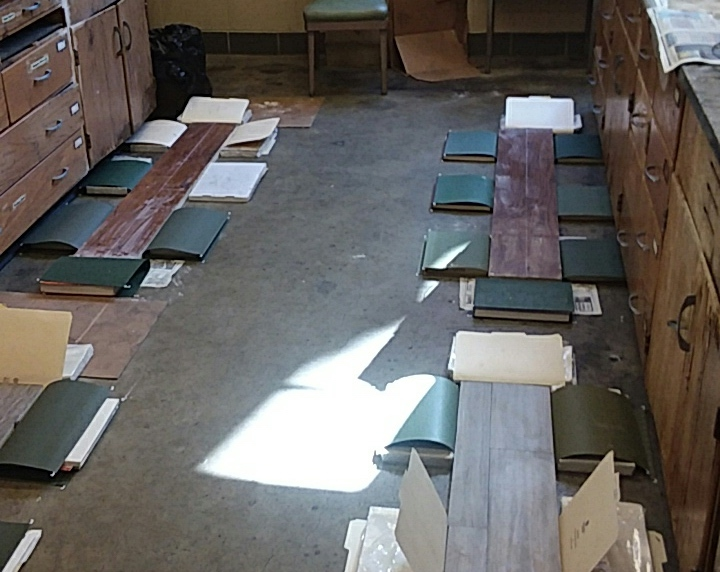
\includegraphics[scale=.2]{Path2}
\caption{This is what the path will look like when set up.}
\label{Figure 1}
\end{figure}

3. To insure a natural first step, measure 48 cm from the front end of each board. This is were the heel hits for the second step of a 5 foot 7 inch individual. From that point measure the first 33cm of the board. This will be the area we cover in the dusting medium. (Please measure the stride and shoe of the person that will be stepping for a more exact measurement.) \textbf{Note} If you would like to reuse the dusting medium, place a piece of newspaper under the area to be dusted. This will capture the powder and allow it to be re-used.

4. At this point, have another technician hold a barrier around the designated spot.This will once again insure that the dusting medium does not spill over into the surrounding area. \textbf{Note}This is not vital but the clouds of dust will settle over the entire area.

5. Using the listed applicator method from above, carefully dust a thin layer of the medium onto the barred off area. When you are finished, remove the barrier. Repeat this for the front of every board.

6. Have the technician that will be taking the prints put on the desired shoes and stand in front of either the right side board or the left.

7. Their first step will be with the foot we are not interested in printing. Their first step will be on the clean flooring while their second will be into the medium. With a normal stride, they will step up onto the board and walk down the path. Only the shoe of interest should be touching the flooring. The other foot will walk along the raised books that had been placed earlier.  You should get three prints per board. Once off the vinyl path, step onto the wood path and follow the same procedure. When finished, step into the mat at the end.

7. At this point, take off the completed shoe and repeat the procedure for the other shoe.

\subsection{Baby Powder Print Photography}

1. Make sure that all shades are drawn and that any windows without shades have been covered.

2. Photograph all prints in high definition. Using the photography cart (Figure 2-3) (please refer to the High Resolution Photography and Camera Equipment: Procedure), position the camera about 1 foot above the print.

\begin{figure}[!htp]
\centering
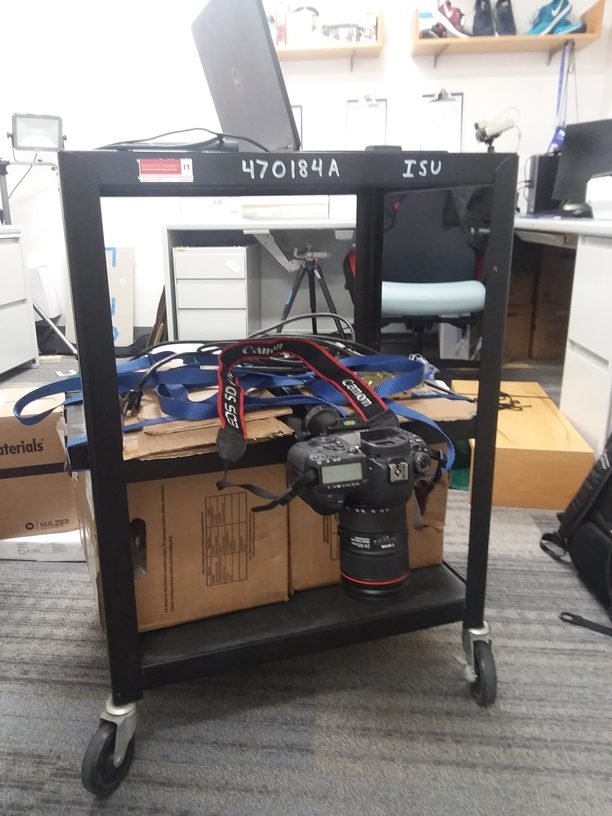
\includegraphics[scale=.2]{Cart1}
\caption{This is the camera cart to be used during this procedure. For Full set up instructions, please see the High Resolution Photography and Camera Equipment: Procedure }
\label{Figure 2}
\end{figure}

\begin{figure}[!htp]
\centering
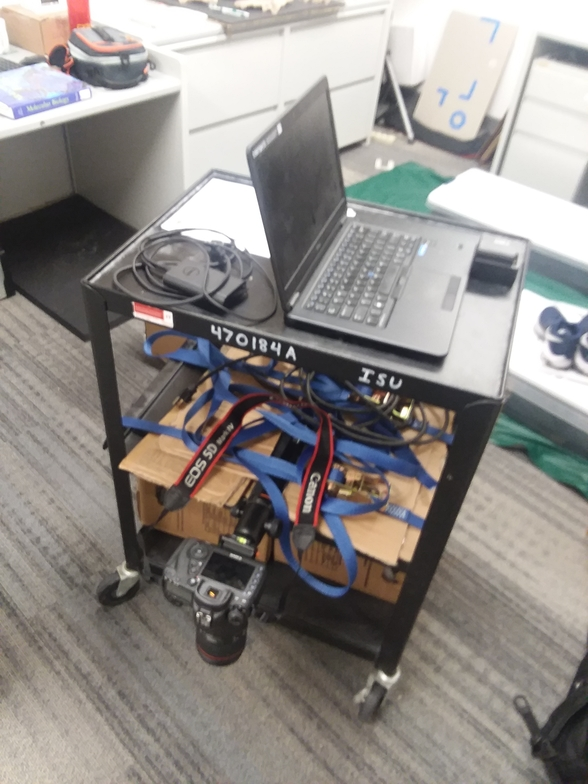
\includegraphics[scale=.2]{Cart2}
\caption{This is the camera cart to be used during this procedure. For Full set up instructions, please see the High Resolution Photography and Camera Equipment: Procedure }
\label{Figure 3}
\end{figure}

3. Making sure that the camera is turned off, plug the USB cable into the camera body (left side). Do not force the plug or the screw into the camera. Plug the other end into the back of the laptop.

4. Remove the lens cap and turn on the camera by sliding the switch located on the upper left-hand side of the camera from Off to On

5. The computer currently opens the following:
•	Control panel/hardware and sound/devices and printers/canon EOS 5d mark IV
i.	this window can be closed
•	EOS utility 3
ii.	if this program does not start you can manually start it

6. To remotely take pictures, select “remote shooting”

7. The pop up that comes up is used to control the camera. Select “live view” on this same menu

8. Being careful not to disturb the powder, place the L-shaped ruler next to the shoe print such that the heel of the shoe print is open. Make sure that the ruler is flat and not covering any portion of the print. Turn off the room lights.

10. There will be three prints on each board. Despite differences, all prints will be handled the same way. Three different images per print. For print one, place a Night Stick both above and below the print, setting them on the previously placed books when convenient. They will be at half power. Adjust the camera so that the entire thing is level and the entire scale and print are in the image. If all is visible, select the acquire button located on the main control panel (Figure 4-5).

\begin{figure}[!htp]
\centering
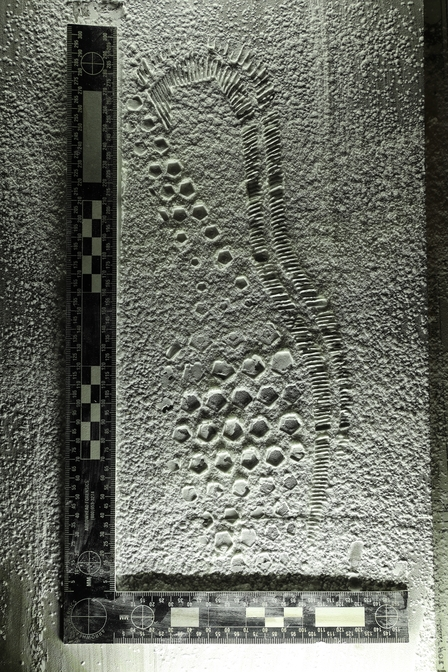
\includegraphics[scale=1.3, angle=180]{Vinyl1.png}
\caption{This is an example of a negative Photo replicate 1 on vinyl flooring}
\label{Figure 4}
\end{figure}

\begin{figure}[!htp]
\centering
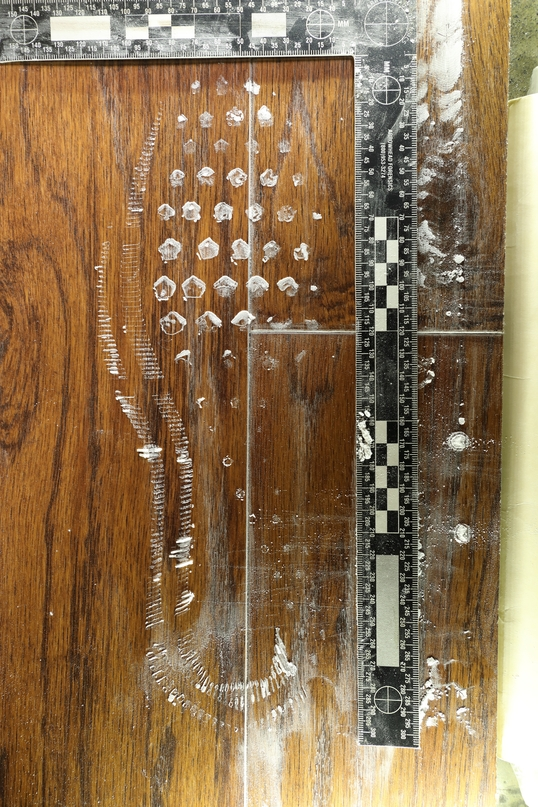
\includegraphics[scale=1.3]{Wood1.png}
\caption{This is an example of a step photo replicate 1 on wood flooring }
\label{Figure 5}
\end{figure}

\newpage

11. Properly name and save the image to the desired folder on the desktop, cybox, or shared drive.

12. For the second image, place the Night Sicks on the left and right sides of the print. They will be at half power. Focus the camera again. If all is visible, select the acquire button located on the main control panel (Figure 7-8).

\begin{figure}[!htp]
\centering
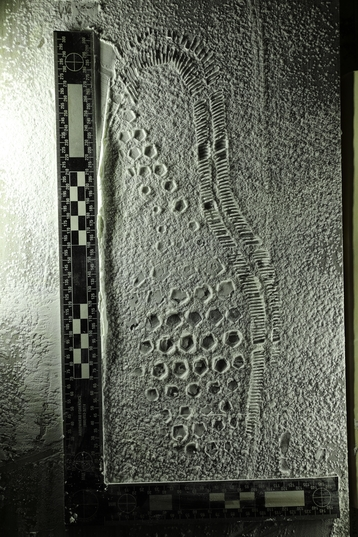
\includegraphics[scale=1.8, angle=180]{Vinyl2.png}
\caption{This is an example of a negative Photo replicate 2 on vinyl flooring}
\label{Figure 6}
\end{figure}

\begin{figure}[!htp]
\centering
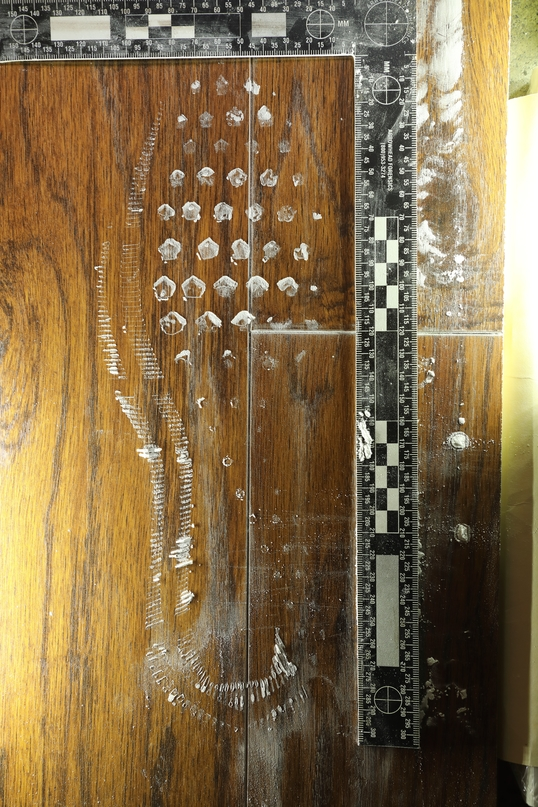
\includegraphics[scale=1.3]{Wood2.png}
\caption{This is an example of a step photo replicate 2 on wood flooring }
\label{Figure 7}
\end{figure}

\newpage

13. Properly name and save the image to the desired folder on the desktop, cybox, or shared drive.

14. For the third image, turn off the Nigh Sticks and turn on the room lights. This image will be taken using normal ambient lighting. Focus the camera again.  If all is visible, select the acquire button located on the main control panel (Figure 7-8).

\begin{figure}[!htp]
\centering
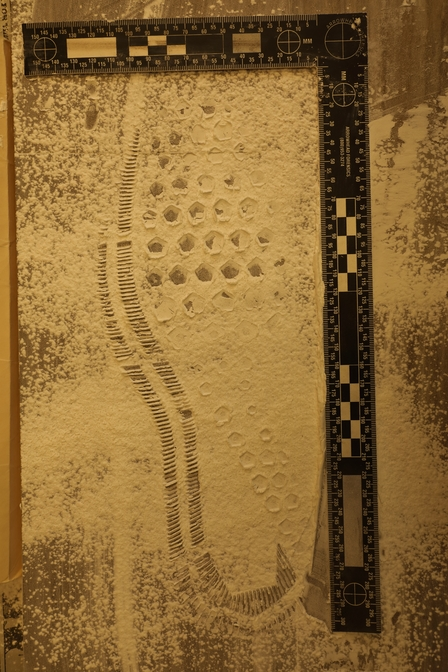
\includegraphics[scale=1.3]{Vinyl3.png}
\caption{This is an example of a negative Photo replicate 3 on vinyl flooring}
\label{Figure 8}
\end{figure}

\begin{figure}[!htp]
\centering
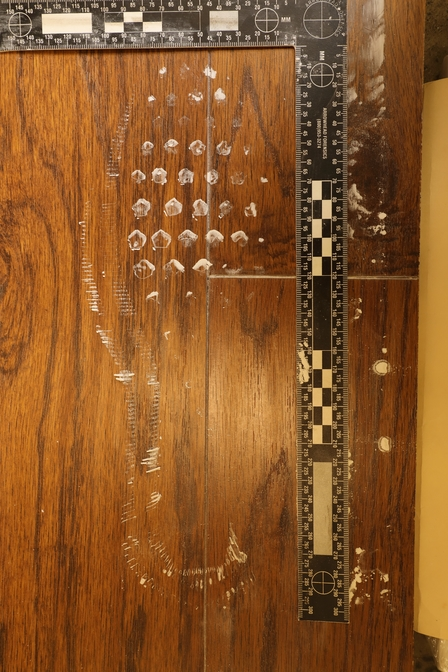
\includegraphics[scale=1.3]{Wood3.png}
\caption{This is an example of a step photo replicate 3 on wood flooring }
\label{Figure 9}
\end{figure}

15. Properly name and save the image to the desired folder on the desktop, cybox, or shared drive.

16. Repeat these steps for each of the 12 prints that are created for each pair of shoes. When finished, there will be 36 images per pair.




\end{document}
